\section{Presentation of experimental or analytical results/descriptions of final constructed product}

在这一部分,我们将讨论我们的模型的测试结果,并探索进一步改进的领域。

\subsection{在测试集上验证模型的准确性}

训练后,我们在一个特别准备的测试集上评估了模型的准确性。准确性定义为模型预测与实际标签匹配的样本比例。

下面的表格和图形展示了模型在不同类别中的准确性:

\begin{figure}[htbp]
    \centering
    \begin{minipage}{0.45\textwidth}
        \centering
        \captionof{table}{Model accuracy on test set}
        \begin{tabular}{cc}
            \toprule
            Category & Accuracy(\%) \\
            \midrule
            Normal & 98.4 \\
            Horizontal Line & 95.6 \\
            Vertical Line & 80.0 \\
            Slope & 96.1 \\
            Other & 95.2 \\
            \bottomrule
        \end{tabular}
        \label{tab:model_accuracy}
    \end{minipage}
    \begin{minipage}{0.45\textwidth}
        \centering
        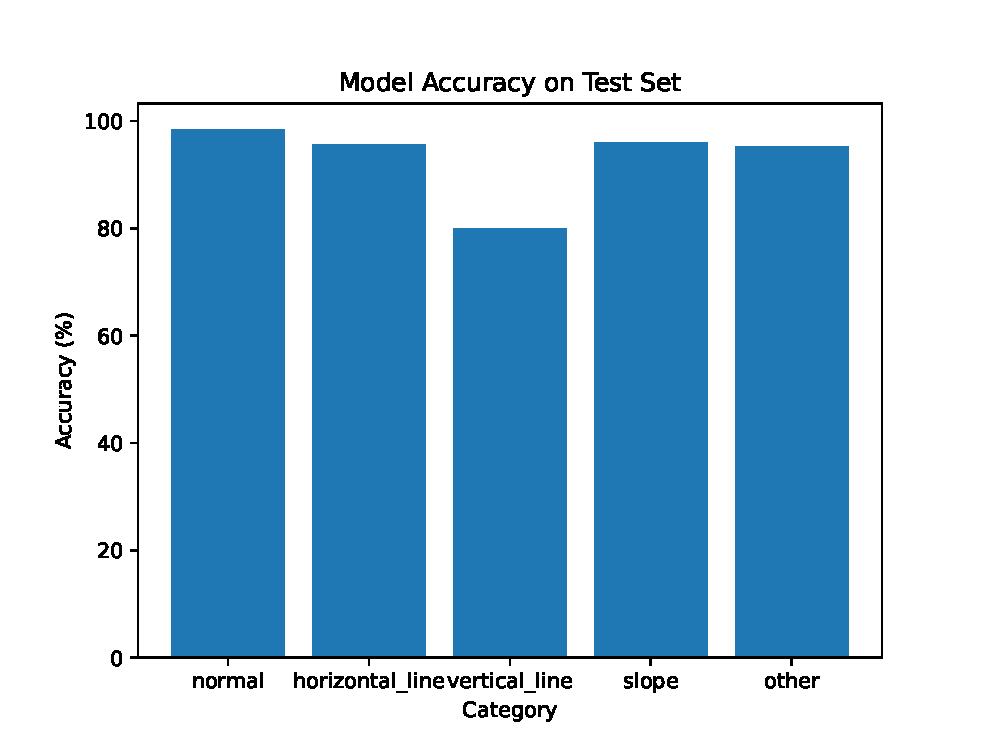
\includegraphics[width=\textwidth]{./fig/assistplot/accuracy.eps}
        \captionof{figure}{Accuracy on Test Set}
        \label{fig:accuracy_histogram}
    \end{minipage}
\end{figure}


\textbf{模型性能分析}

模型在"正常"类别中的表现非常出色,准确率达到98.4%,这表明它在识别没有明显缺陷的组织切片方面具有强大的能力。同样,"水平线"和"其他"类别的准确度也很高,反映出模型在识别这些特定类型的缺陷方面的有效性。

然而,"垂直线"类别的准确度明显较低,只有80.0%。这表明模型识别这种类型缺陷的能力需要加强。这可能是由于训练数据不足,限制了模型的学习。也可能是因为垂直线的特征相对不太明显,使得模型难以准确提取特征。

\subsection{模型的改进(改变输入分辨率)}

在这里,我们将讨论模型进一步改进的可能性。

将高分辨率图像缩放到InceptionV3模型所需的默认大小299x299,确实可能导致信息和细节的丢失。这对于原始分辨率较高的图像尤其关键,例如VHX7000设备拍摄的2880x2160的图像。直接缩小这些图像可能会阻碍模型捕获所有微妙差异的能力,这在医学成像等细节丰富至关重要的领域尤其有害。

一种可能的解决方案是修改模型的输入层,以接受更大的图像尺寸。这种方法使模型能够处理更高分辨率的图像,从而保留更多的原始信息和细节,这可能会提高性能和准确度。InceptionV3架构,其具有多个不同核大小的卷积,特别适合处理更大的图像,因为它可以有效地捕获不同尺度的特征。

由于实验室硬件(16GB的显存)的限制,图像被缩放到原始大小的0.4倍,因此在这个实验中,图像的尺寸为1152x864。

\textbf{Training the New Model (Model 4)}

Model 4 is trained with these adjusted image sizes, and its training effectiveness is as follows:

\begin{figure}[H]
    \centering
    \begin{minipage}{0.45\textwidth}
        \centering
        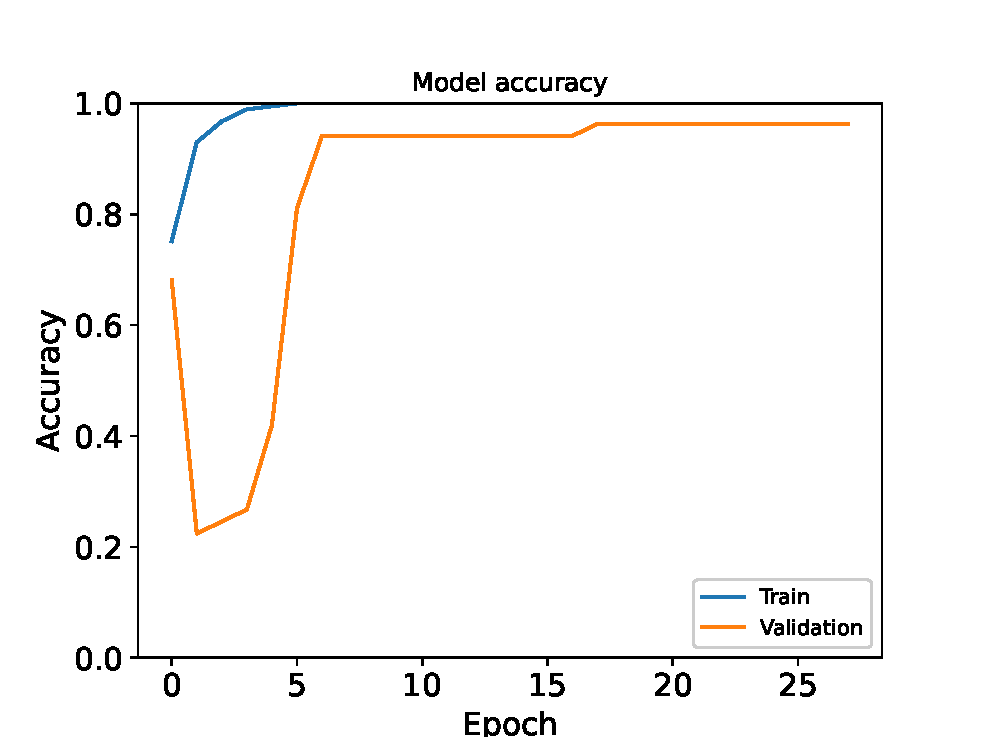
\includegraphics[width=\textwidth]{./fig/model4/accuracy4.eps}
        \caption{Model-4 accuracy}
        \label{fig:model4_accuracy}
    \end{minipage}
    \begin{minipage}{0.45\textwidth}
        \centering
        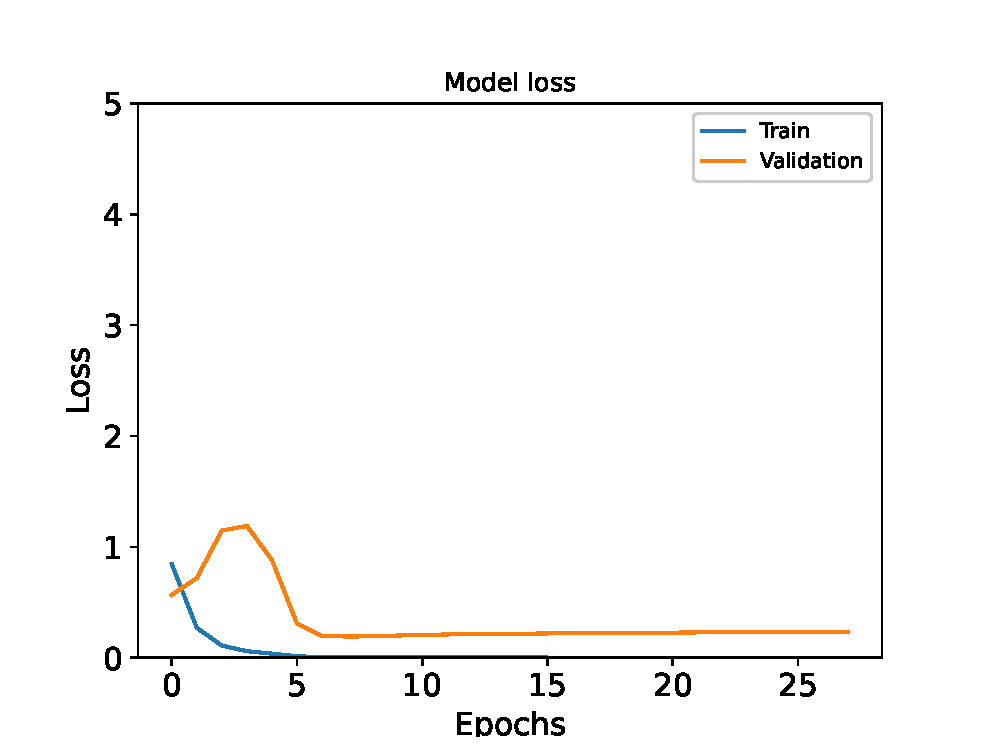
\includegraphics[width=\textwidth]{./fig/model4/loss4.eps}
        \caption{Model-4 loss}
        \label{fig:model4_loss}
    \end{minipage}
\end{figure}

通过观察训练准确性和损失随时间的变化,我们可以看到模型性能有了显著的提升。训练和验证的准确性都接近1,验证损失降低到大约0.2,这表明模型具有强大的泛化能力。这表明模型不仅在训练数据上表现优秀,而且能够有效地泛化到新的、未见过的数据。

\textbf{在测试集上重新评估准确性}

更新后的模型然后在测试集上重新进行评估,结果如\autoref{tab:model_accuracy2}所示:

\begin{table}[H]
    \centering
    \caption{model accuracy on test set}
    \begin{tabular}{cccccc}
        \toprule
        & normal & horizental\_line & vertical\_line & slope & other \\
        \midrule
        accuracy(\%) & 98.4 & 96.7 & 85.6 & 96.5 & 96.5 \\
        \bottomrule
    \end{tabular}
    \label{tab:model_accuracy2}
    \end{table}

比较改变分辨率前后的准确性,有明显的提升,尽管不是很大。这种适度的增加可能归因于已经接近1的高准确性,进一步的改进有递减的回报。

结果证实了处理高分辨率图像的潜在好处,特别是在需要高保真和细节的设置中,如生物组织分析和研究。

\subsection{研究机器的最佳切割角度}

为了确定微切机的最佳切割角度,我们准备了在8到12度之间,以0.5度为增量的各种角度切割的组织切片图像。每个角度类别包含100个图像,总共有9个不同的数据组。然后使用模型4来评估每组的质量率,目标是找出获得高质量切片最多的角度。

下表和图形展示了每个切割角度的准确性,定义为高质量切割的百分比:

\begin{figure}[H]
    \centering
    \begin{minipage}{0.4\textwidth}
        \centering
        \captionof{table}{Normal accuracy on different angle}
        \begin{tabular}{cc}
            \toprule
            Angle & Accuracy(\%) \\
            \midrule
            8 & 80 \\
            8.5 & 81.5 \\
            9 & 83.5 \\
            9.5 & 93.3 \\
            10 & 96.6 \\
            10.5 & 88.8 \\
            11 & 84.2 \\
            11.5 & 66.6 \\
            12 & 62.2 \\
            \bottomrule
        \end{tabular}
        \label{tab:model_accuracy_angle}
    \end{minipage}
    \begin{minipage}{0.55\textwidth}
        \centering
        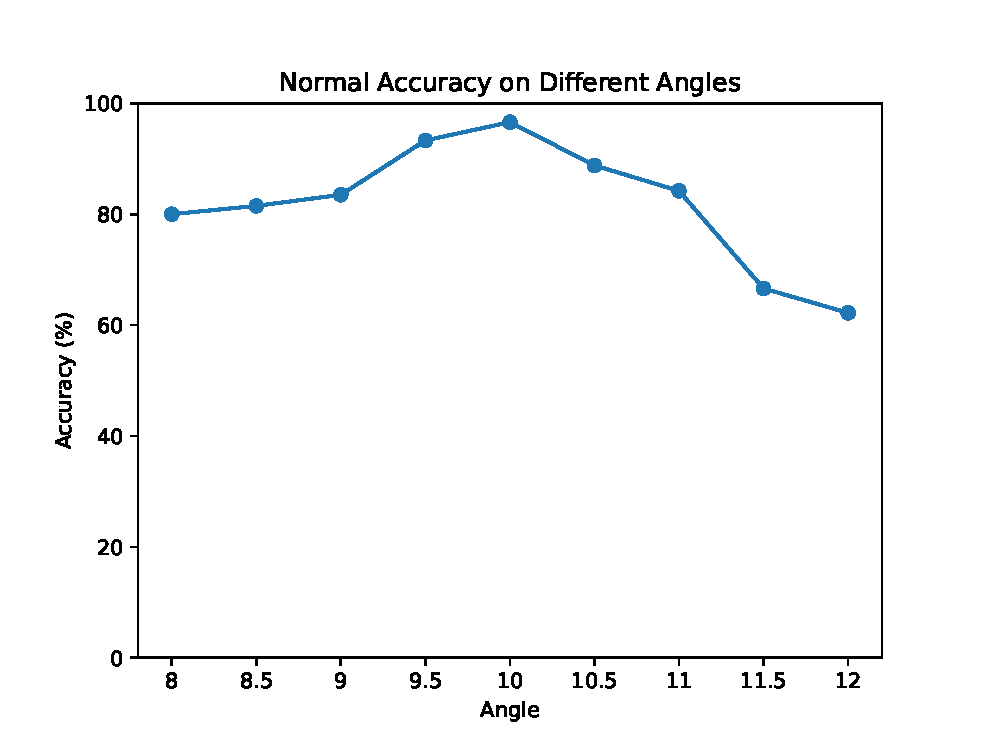
\includegraphics[width=\textwidth]{./fig/assistplot/angle_accuracy.eps}
        \captionof{figure}{Model Accuracy on Different Angle}
        \label{fig:angle_accuracy_histogram}
    \end{minipage}
\end{figure}

从\autoref{tab:model_accuracy_angle}中的数据可以看出,获得最高质量组织切片的最佳切割角度是10度,准确性高达96.6%。

此外,如\autoref{fig:angle_accuracy_histogram}所示,为了保持至少80%的切片质量率,切割角度应设置在9到10.5度之间。这个范围不仅确保了高质量切割的比率,而且还提供了一些机器设置的灵活性,以适应可能的组织类型或条件的变化。

\subsection{模型的泛化性}

到目前为止,实验已经使用了来自鱼类的卵巢组织切片。在实际应用中,我们可能会遇到各种各样的组织样本,包括其他器官或来自不同动物的标本。因此,评估我们的模型在各种组织类型上的泛化能力是至关重要的。

我们已经准备了一个新的数据集,包括鱼类肺部组织切片,分为四类:好、正常、差和其他。这些类别在下面的图中展示:(如\autoref{fig:fish_lung})

\begin{figure}[H]
    \centering
    \begin{minipage}{0.24\textwidth}
        \centering
        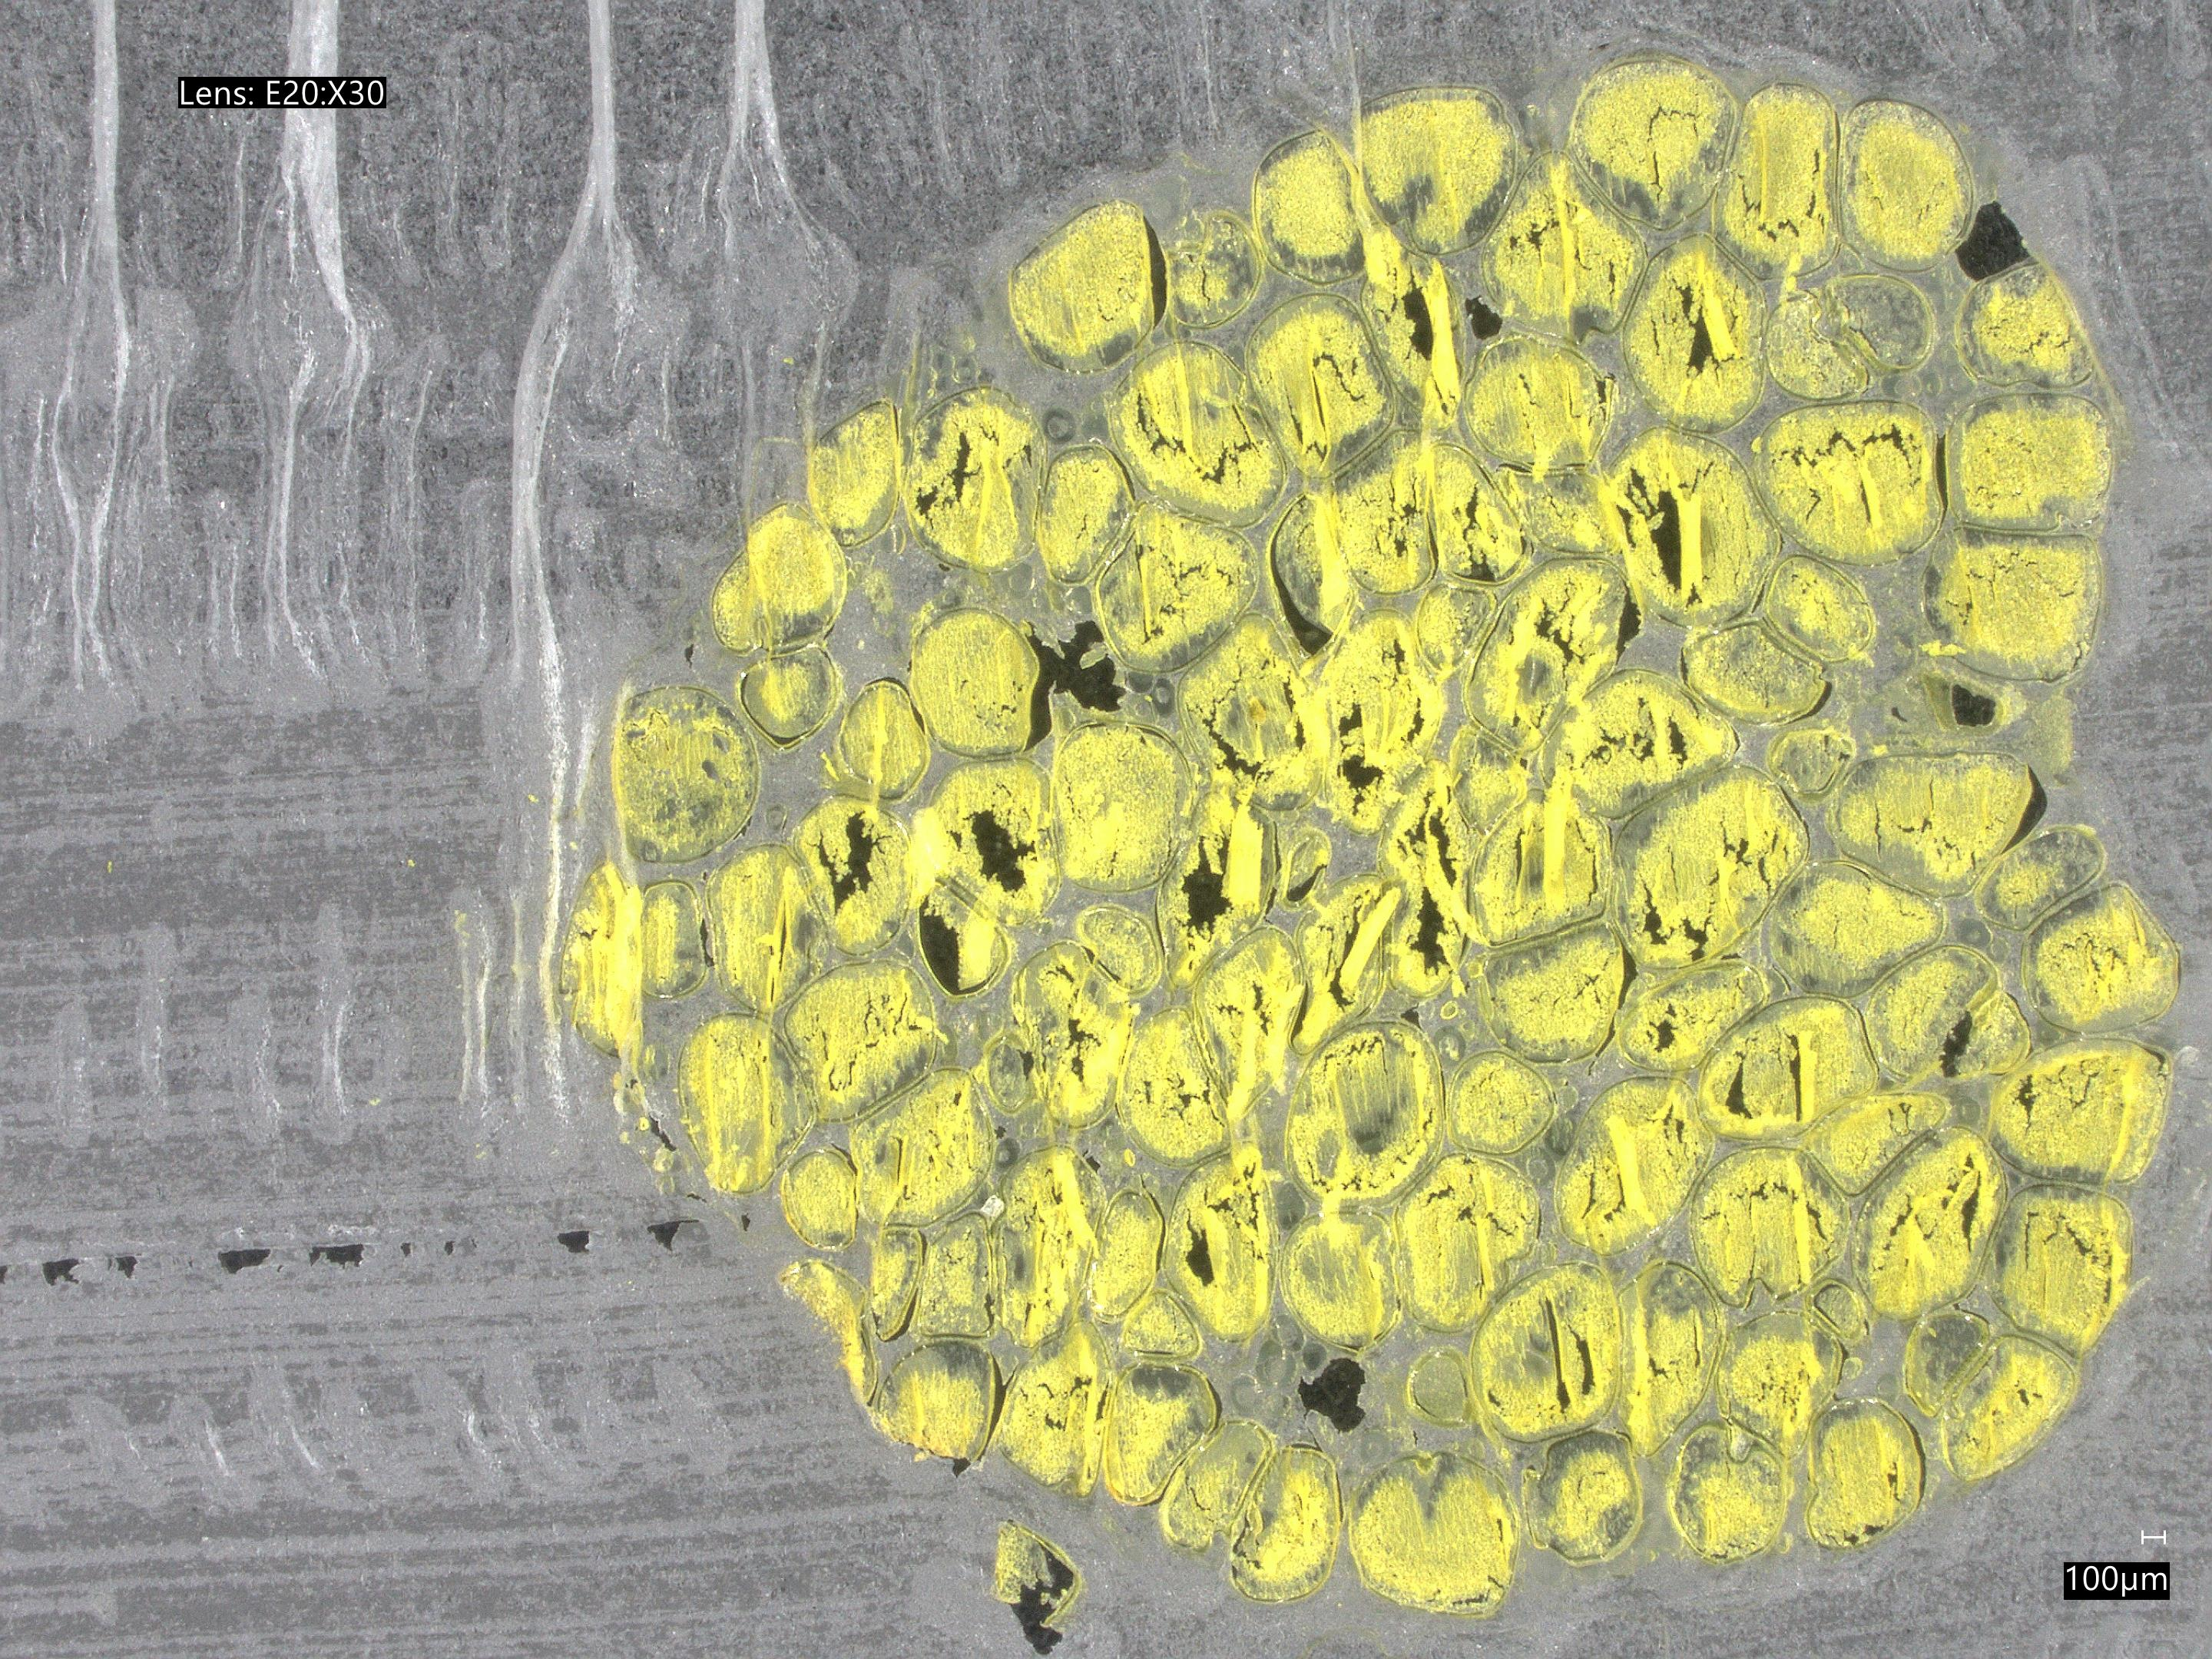
\includegraphics[width=\textwidth]{./fig/fish_lung/good20240313_144138.jpg}
        \caption*{Good}
        % \label{fig:good_fish_lung}
    \end{minipage}
    \begin{minipage}{0.24\textwidth}
        \centering
        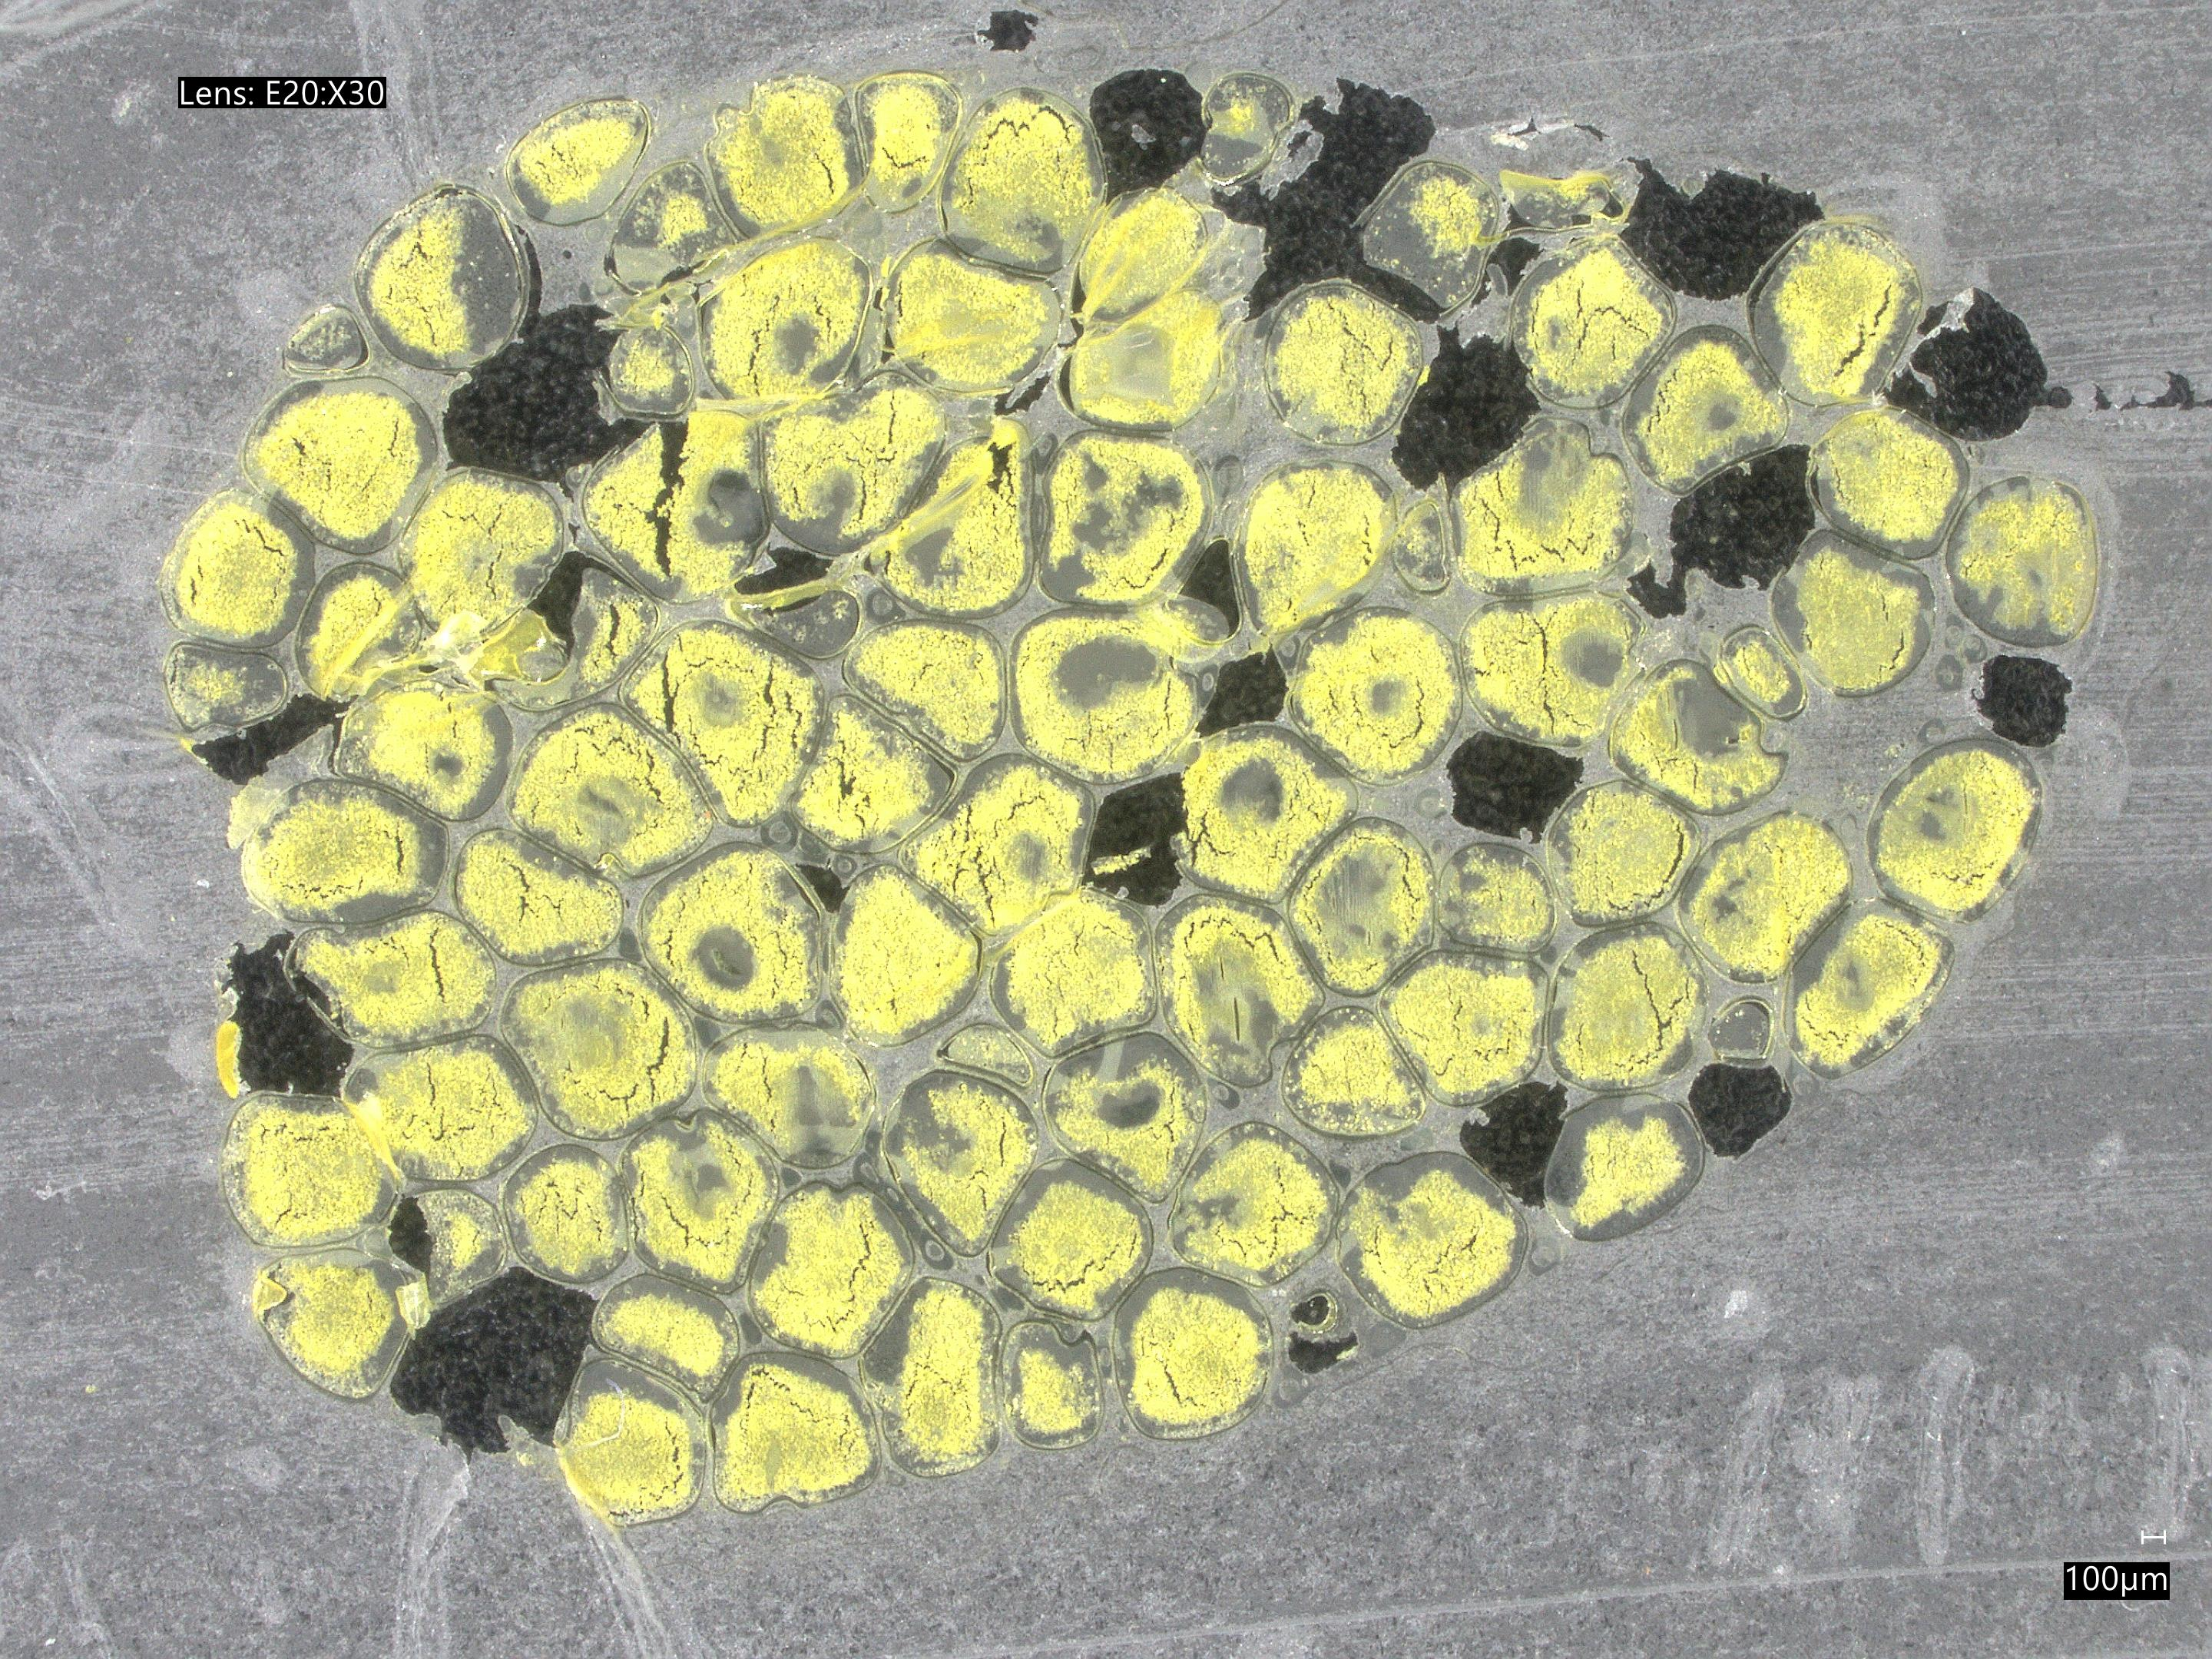
\includegraphics[width=\textwidth]{./fig/fish_lung/normal20240313_141726.jpg}
        \caption*{Normal}
        % \label{fig:noraml_fish_lung}
    \end{minipage}
    \begin{minipage}{0.24\textwidth}
        \centering
        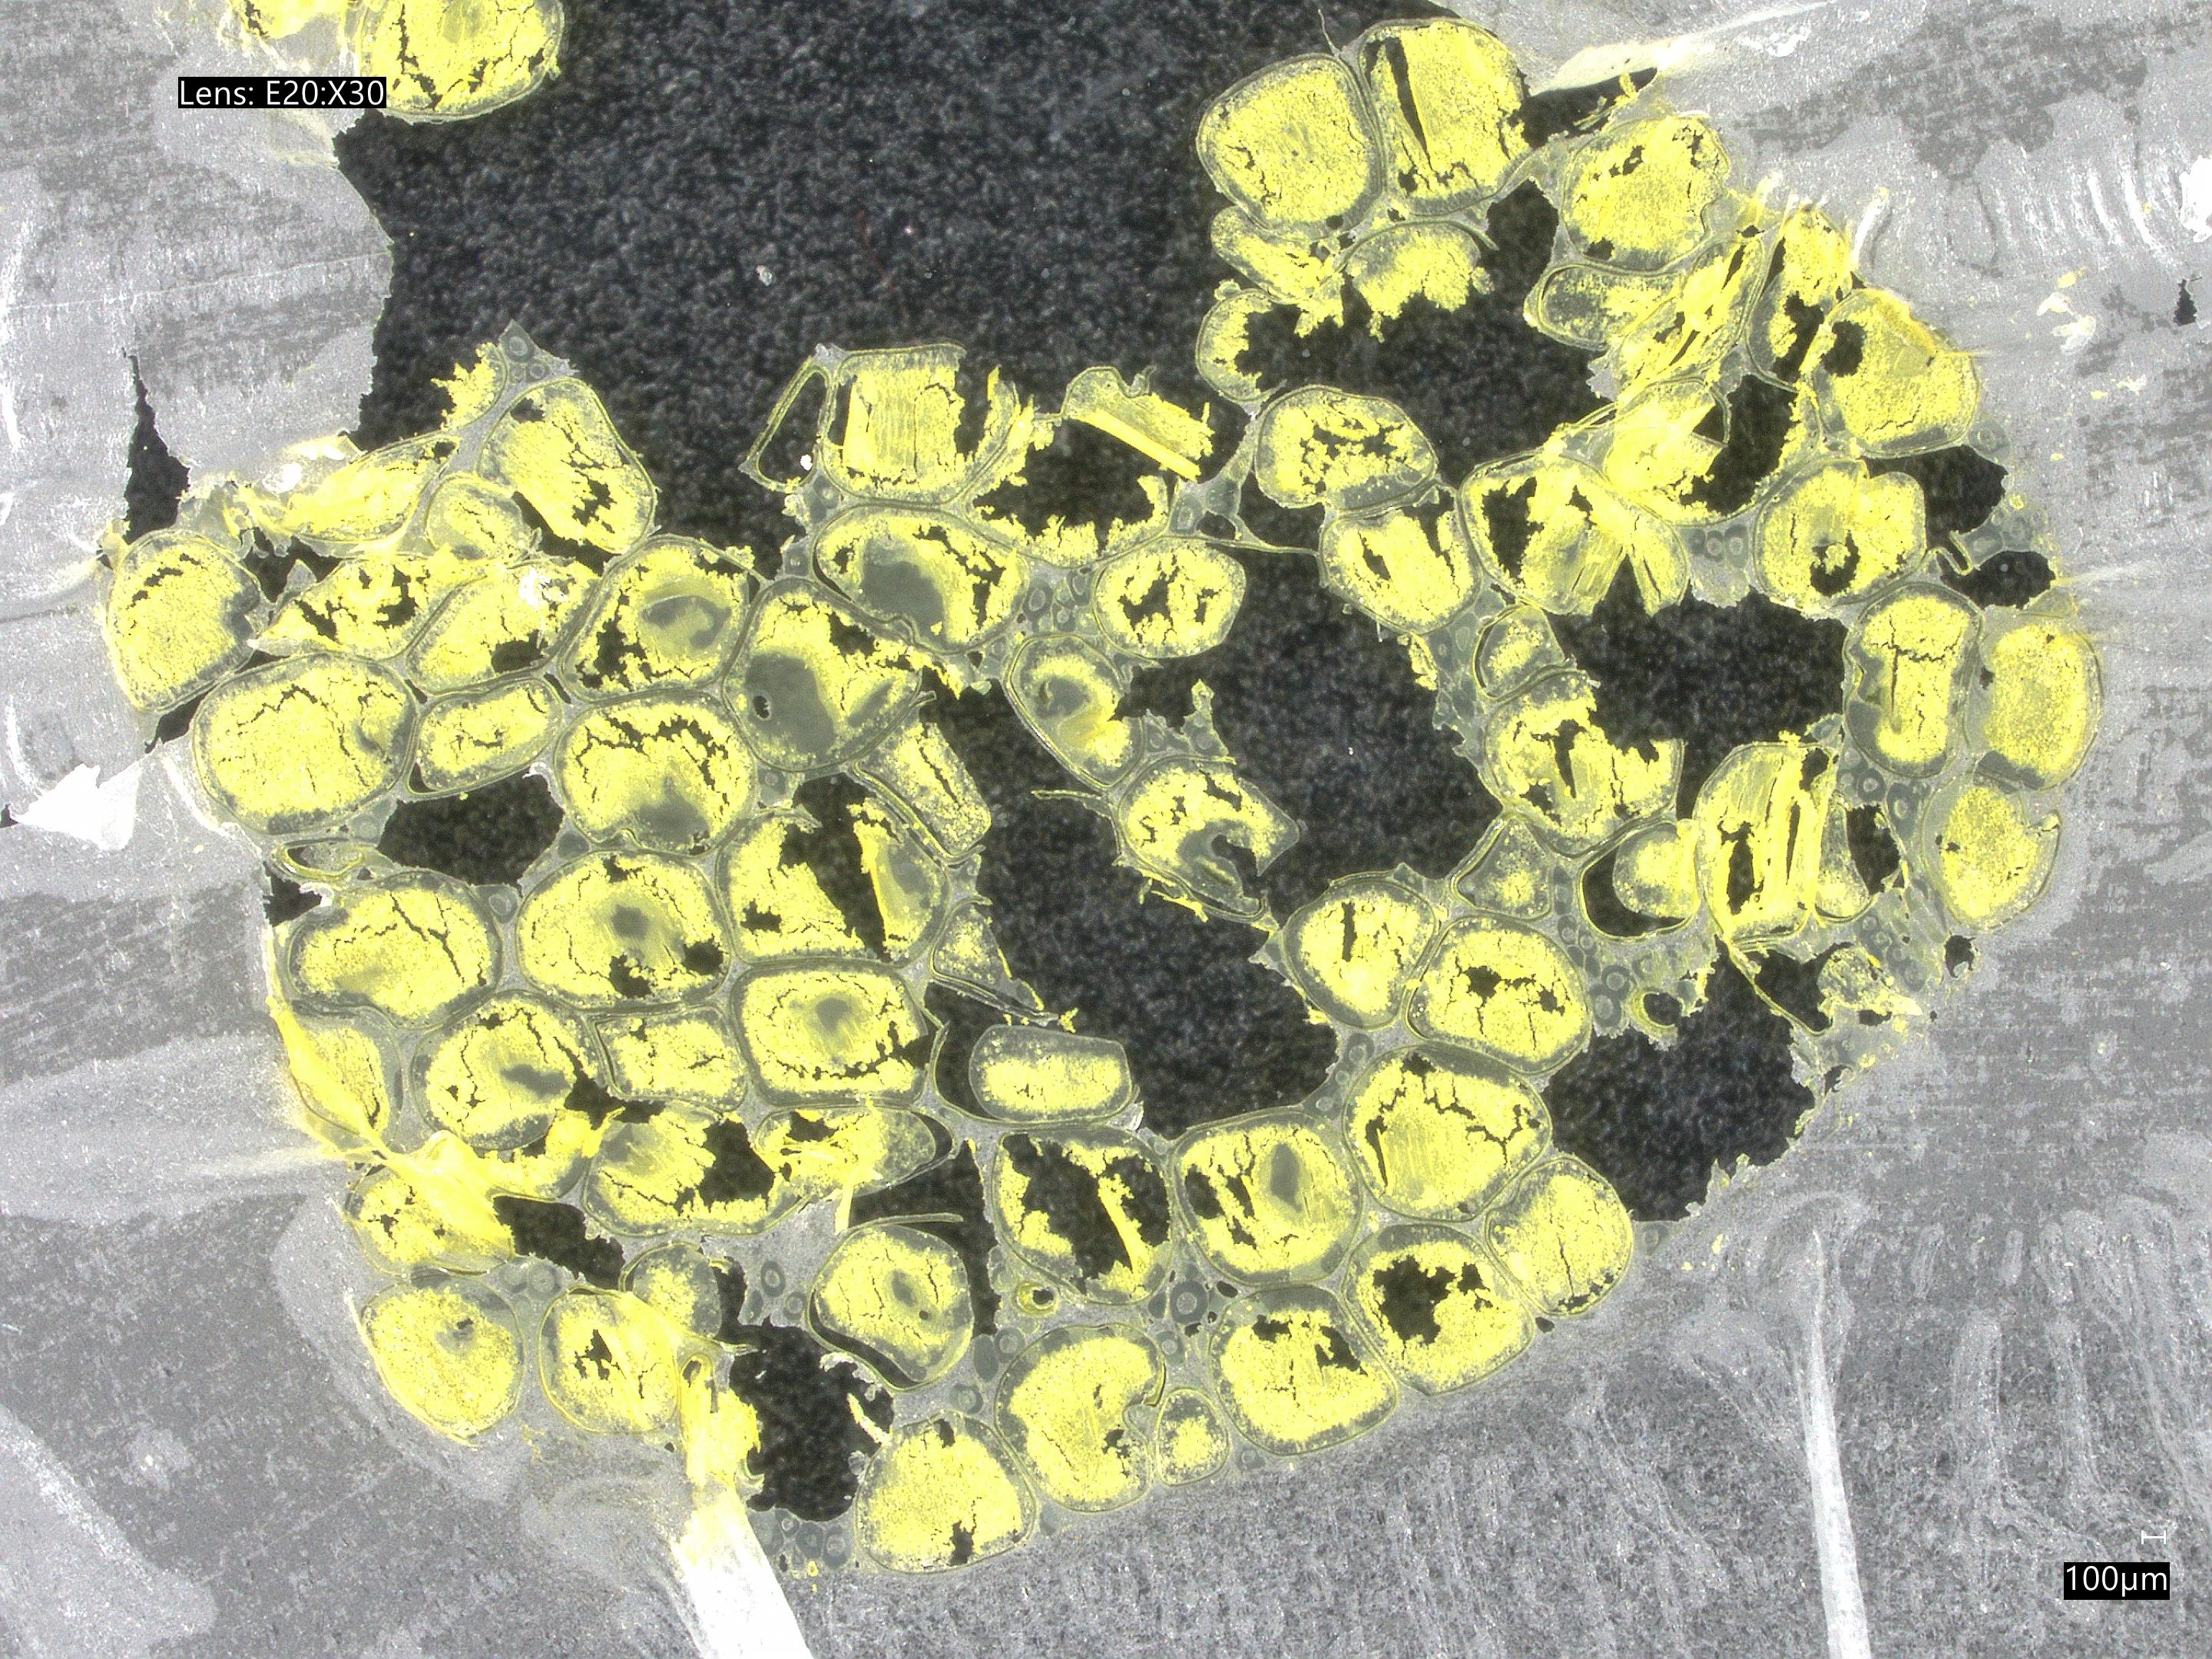
\includegraphics[width=\textwidth]{./fig/fish_lung/bad20240313_140952.jpg}
        \caption*{Bad}
        % \label{fig:bad_fish_lung}
    \end{minipage}
    \begin{minipage}{0.24\textwidth}
        \centering
        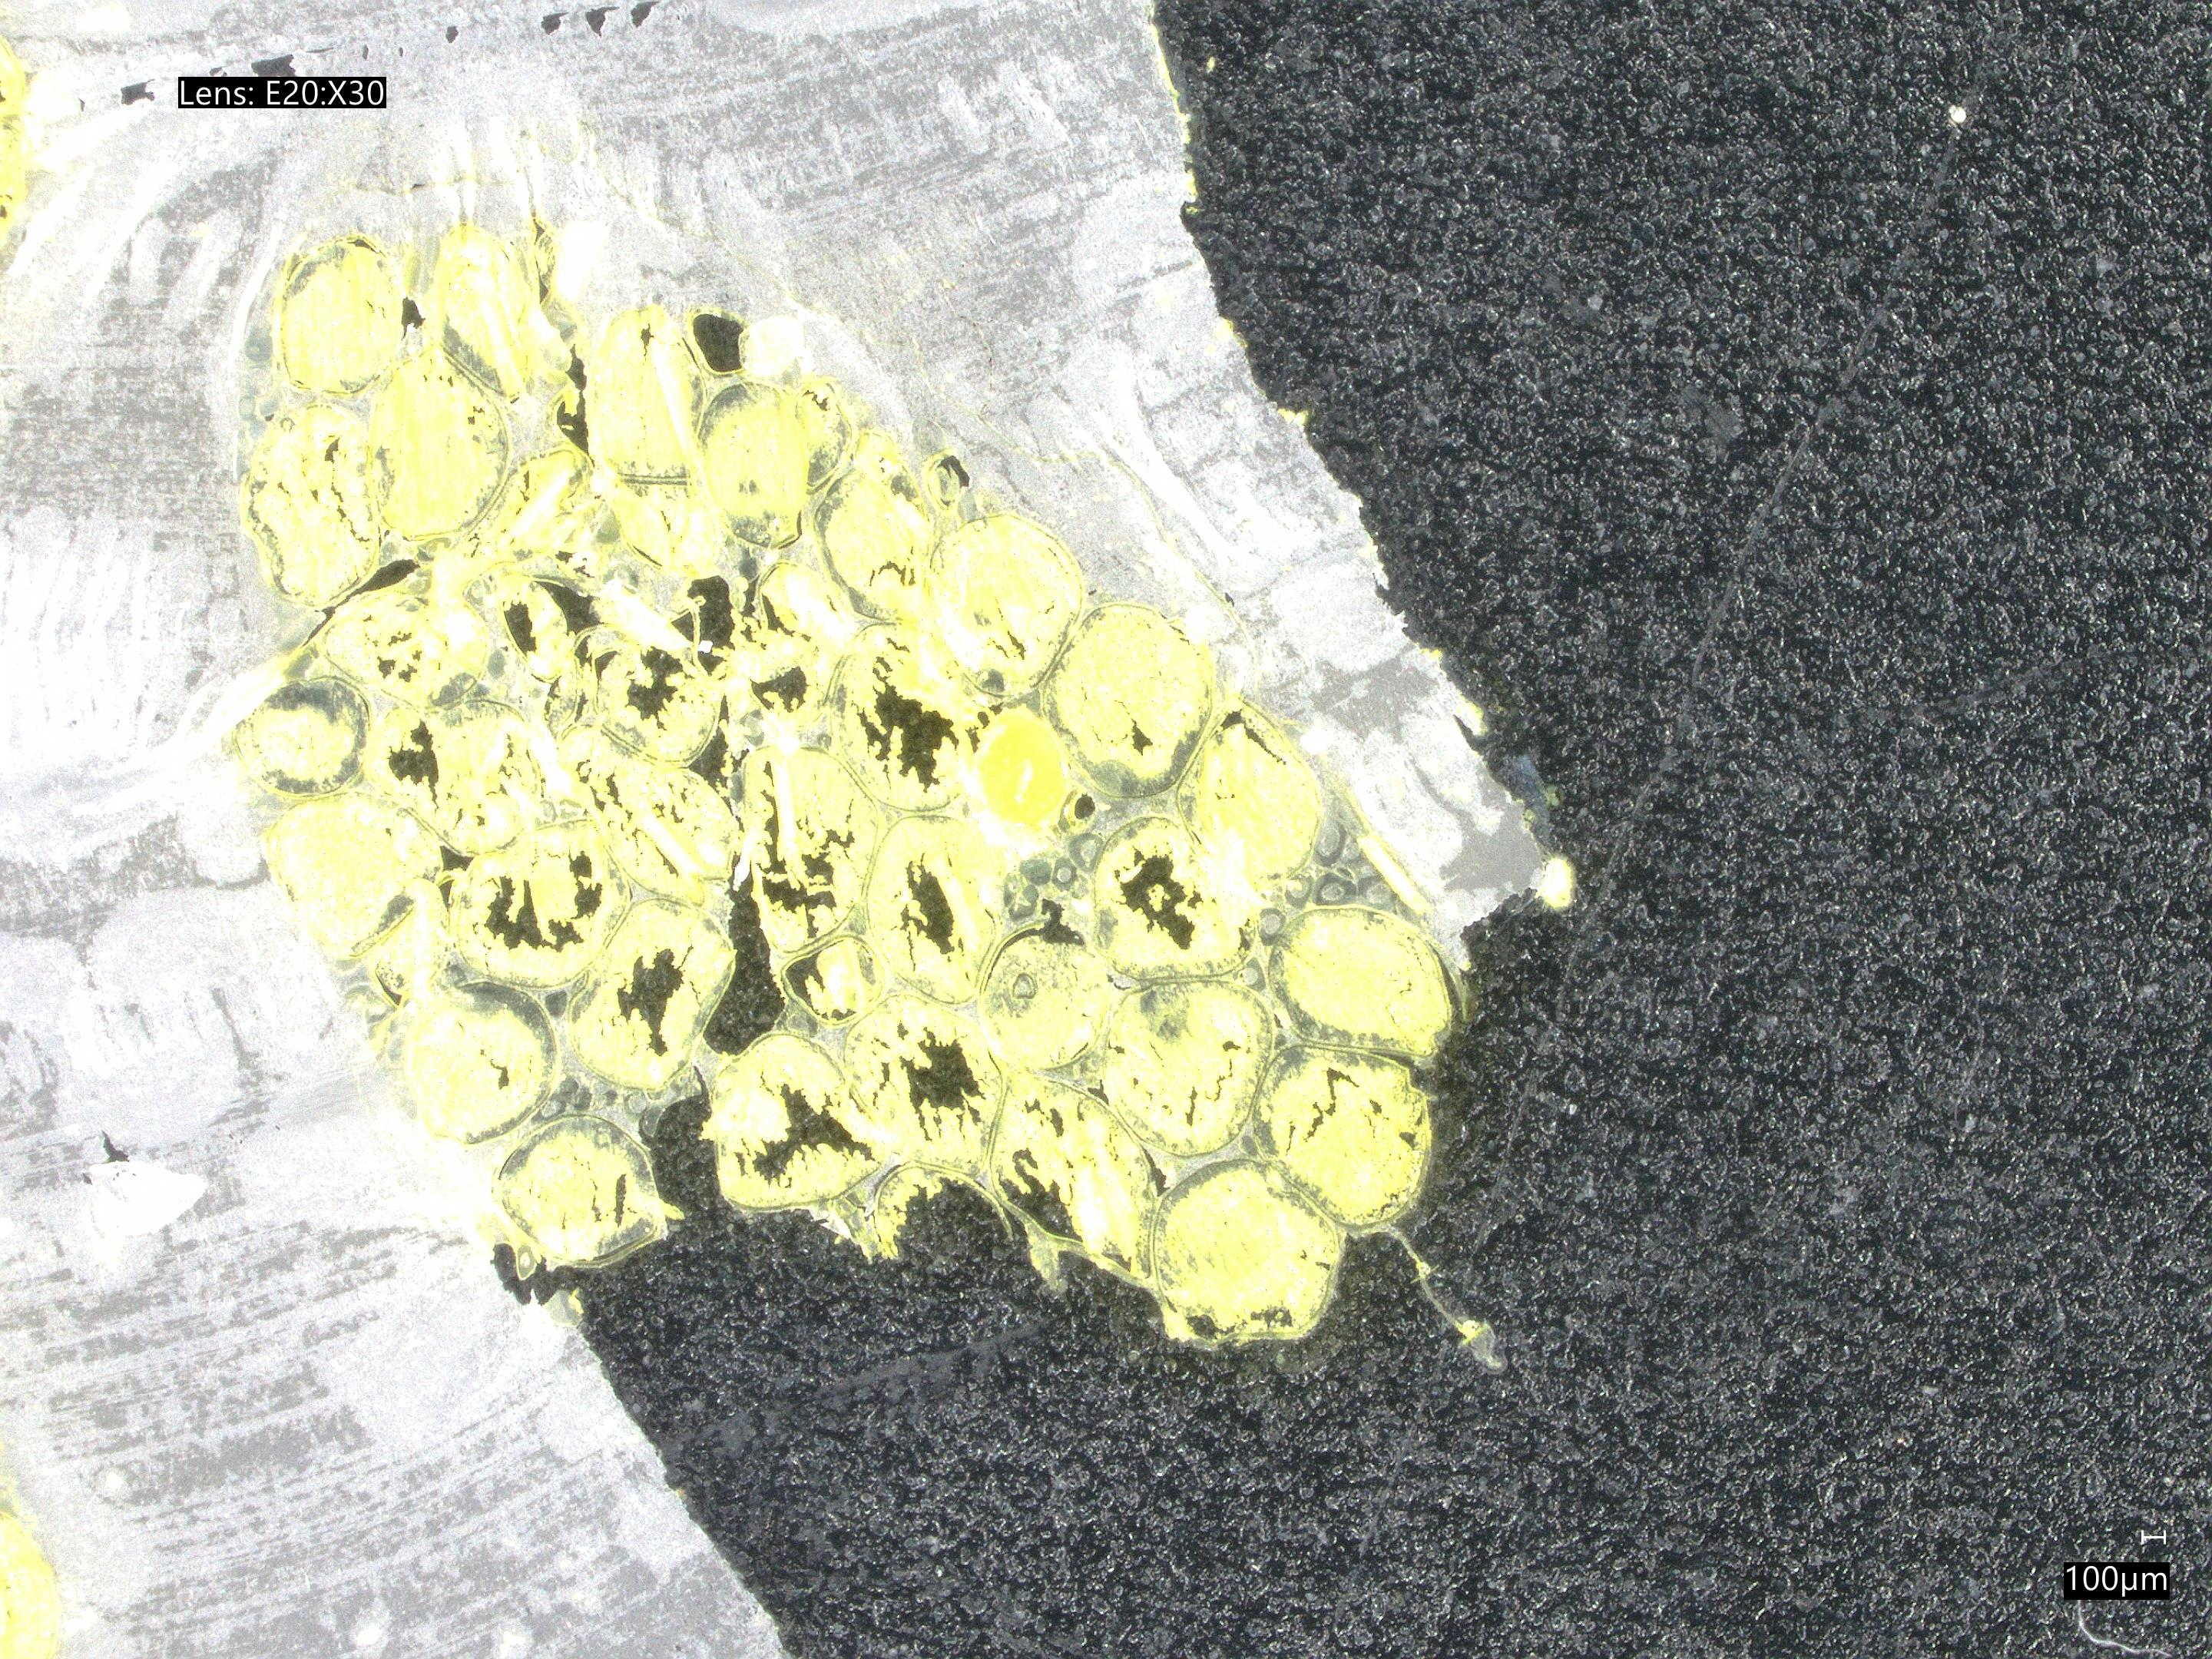
\includegraphics[width=\textwidth]{./fig/fish_lung/other20240313_141858.jpg}
        \caption*{Other}
        % \label{fig:other_fish_lung}
    \end{minipage}
    \caption{Four categories of fish lung tissue}
    \label{fig:fish_lung}
\end{figure}

保持原始的模型架构(模型4),但使用分辨率为1152x864的鱼肺图像重新训练。训练的准确性和损失在\autoref{fig:model5_acc}和\autoref{fig:model5_loss}中展示。
\begin{figure}[H]
    \centering
    \begin{minipage}{0.45\textwidth}
        \centering
        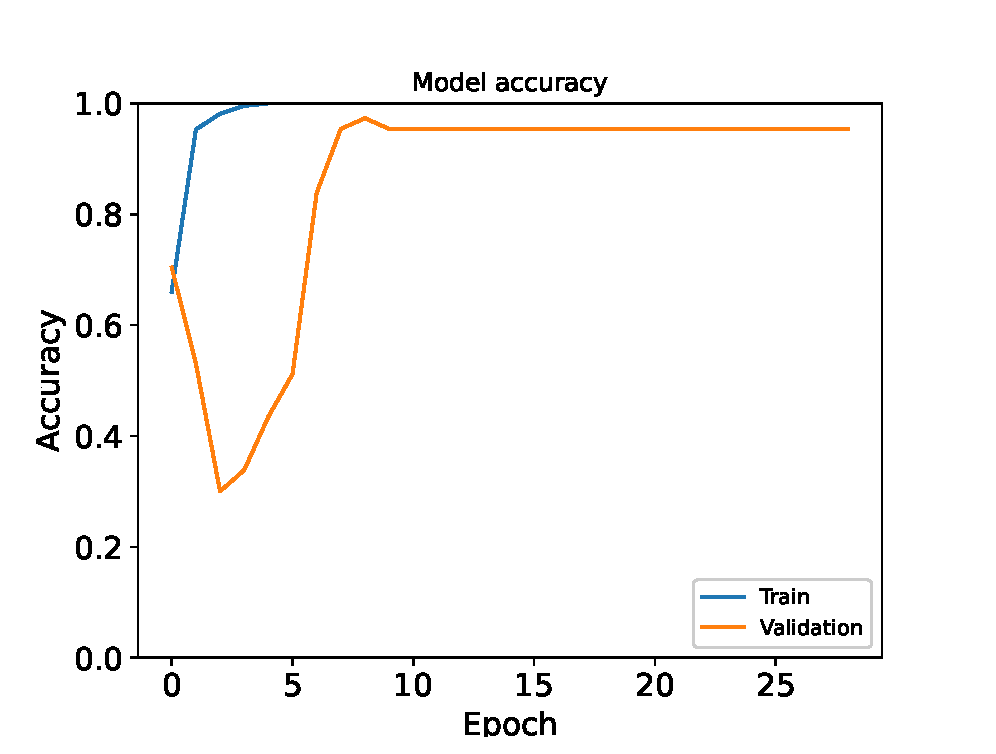
\includegraphics[width=\textwidth]{./fig/fish_lung/accuracy5.eps}
        \caption{Model-5 accuracy}
        \label{fig:model5_acc}
    \end{minipage}
    \begin{minipage}{0.45\textwidth}
        \centering
        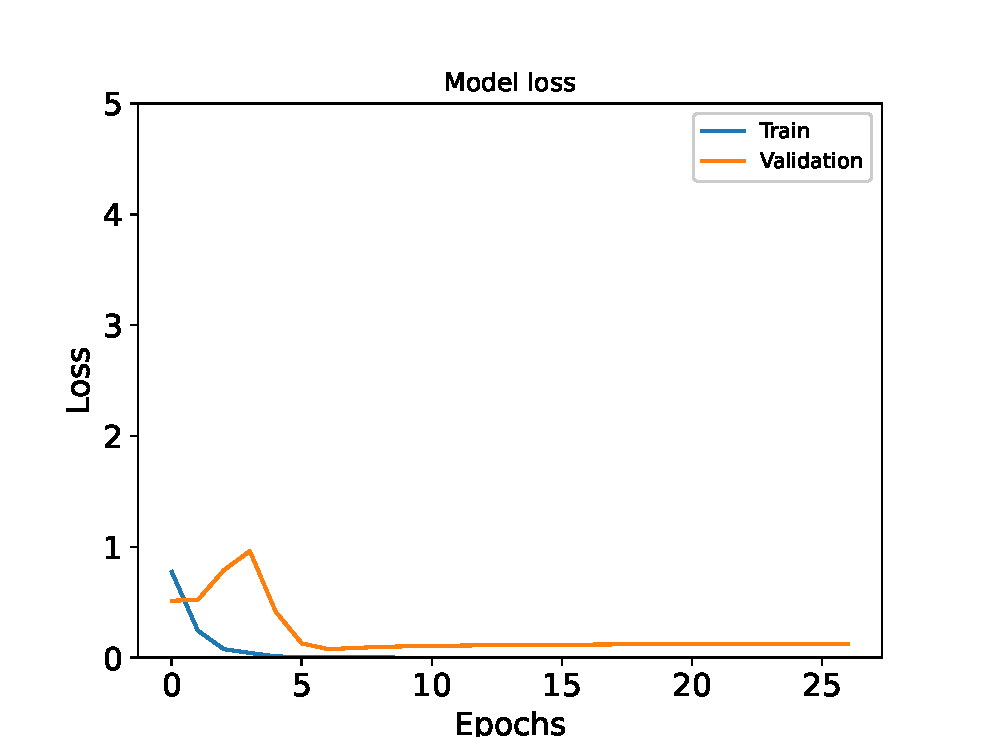
\includegraphics[width=\textwidth]{./fig/fish_lung/loss5.eps}
        \caption{Model-5 loss}
        \label{fig:model5_loss}
    \end{minipage}
\end{figure}

训练和验证的准确性迅速增加并保持在高水平,表明模型在两个数据集上的性能都很强。损失图显示训练损失迅速下降到零,验证损失在初期的激增后稳定下来,这表明模型的拟合和泛化性都很好。

模型进一步在测试集上进行测试,结果显示在\autoref{fig:accuracy_histogram2}中。

\begin{figure}[H]
    \begin{minipage}{0.45\textwidth}
        \centering
        \captionof{table}{Model accuracy on test set}
        \begin{tabular}{ccccc}
            \toprule
            label & accuracy(\%) \\
            \midrule
            bad & 94.1 \\
            good & 98.2 \\
            normal & 94.7 \\
            other & 95.0 \\
            \bottomrule
        \end{tabular}
        \label{tab:model_accuracy3}
    \end{minipage}
    \begin{minipage}{0.45\textwidth}
        \centering
        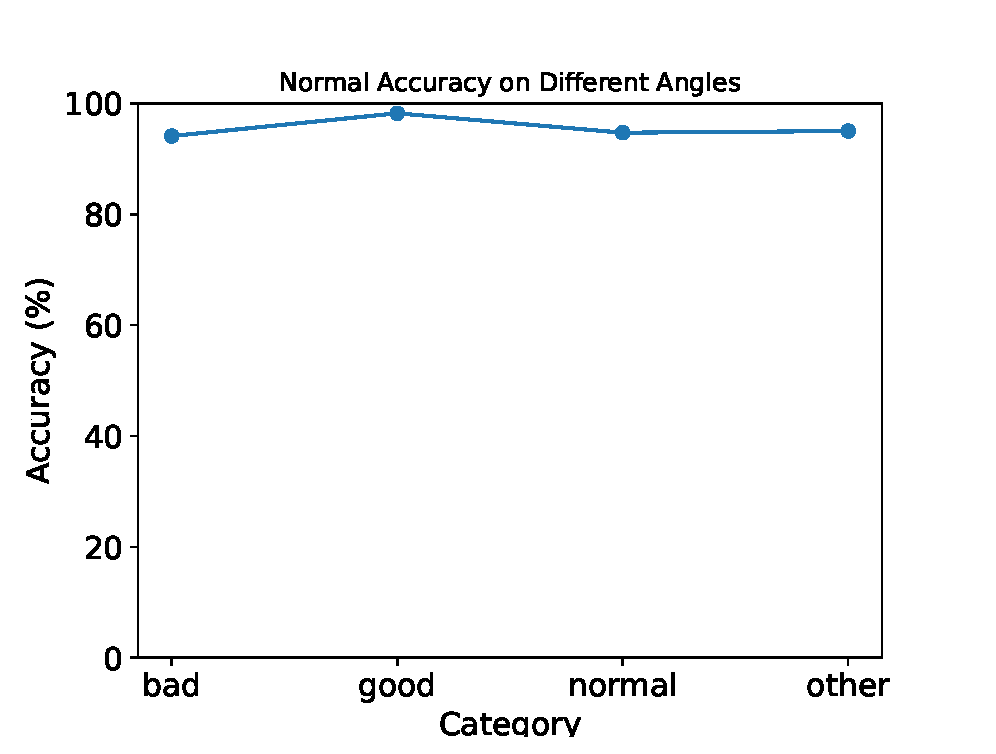
\includegraphics[width=\textwidth]{./fig/assistplot/angle_accuracy2.eps}
        \caption{Accuracy on Test Set}
        \label{fig:accuracy_histogram2}
    \end{minipage}
\end{figure}

该模型在所有标签上的准确率超过90\%,表明其强大的性能和显著的泛化能力。这表明该模型可以有效地分类不同类型的组织切片,可能使其成为各种生物医学成像应用的多功能工具。 模型在不同组织类型上的稳健性强调了其在组织质量评估和分类任务中的潜力。

\FloatBarrier